\documentclass[fr]{../../../../../../eplexam}
\usepackage{listings}
\definecolor{codegreen}{rgb}{0,0.6,0}
\definecolor{codegray}{rgb}{0.5,0.5,0.5}
\definecolor{codepurple}{rgb}{0.58,0,0.82}
\definecolor{backcolour}{rgb}{1.0,1.0,1.0}
\definecolor{codeblue}{rgb}{0,0,0.8}

\lstdefinestyle{mystyle}{
    backgroundcolor=\color{backcolour},   
    commentstyle=\color{codegray},
    keywordstyle=\color{codeblue},
    numberstyle=\tiny\color{codegray},
    stringstyle=\color{codeblue},
    basicstyle=\ttfamily\footnotesize,
    breakatwhitespace=false,         
    breaklines=true,                 
    captionpos=b,                    
    keepspaces=true,                 
    numbers=left,                    
    numbersep=5pt,                  
    showspaces=false,                
    showstringspaces=false,
    showtabs=false,                  
    tabsize=2,
    frame=shadowbox
}
\lstset{style=mystyle}
\lstset{language=Oz}
\hypertitle{}{4}{INFO}{1104}{2021}{Septembre}{All}
{Norah Habets \and Thomas Debelle}
{P. Van Roy}


\section{Scope}
Define the scope of an identifier occurrence. Give a code example where the same identifier occurs more than once and where these occurrences represent more than one variable.

\begin{solution}
La portée d'un identificateur est la partie où l'occurrence se réfère à la même déclaration de variable
\begin{lstlisting}[escapechar=µ]
local
  X
in
  X=42 {Browse X} %Affiche 42
  local
    X
  in
    X=11 {Browse X} %Affiche 11
  end 
  {Browse X} %Affiche 42
end
\end{lstlisting}
\end{solution}

\section{Ordered binary tree}
Define an ordered binarytree type. Give first the EBNF grammar definition Ofa binary tree and then define the condition of bein ordered.

\begin{solution}
EBNF = Extended Backus-Naur form
\begin{lstlisting}[escapechar=µ]
<tree T> ::= leaf|t(T <tree T> ... <tree T>)
<obtree T> ::= leaf|t(key:T value:T left:<obtree T> right:<obtree T>
\end{lstlisting}
\begin{itemize}
\item \underline{Binary:} chaque élément hormis les feuilles ont 2 sous-arbres
\item \underline{Ordered:} pour chaque arbre (inclus les sous-arbres) toutes les clés à gauche dans le sous-arbres sont inférieurs à la clé de la racine. Les clés à droite sont toutes supérieures à celles de la clé de la racine.
\end{itemize}
\end{solution}

\section{Deleting a node from an ordered  binary tree}
Given an ordered binary tree where each node has a key and a value. Define the function \{Delete K T\} that removes the node with key K from the tree (if the node exists) and returns a new ordered binary tree that contains all the nodes of T without the node with key K. To implementthe Delete function, you will need to define one auxiliary function, \{RemoveSmaIlest T\} which returns the smallest element of T and a new ordered tree without the smallest element. Both functions should be written in Oz in the declarative paradigm and using pattern matching to keep them simple. To make sure you define Delete and RemoveSmaIIest correctly, it can be a good idea to draw diagrams of what these functions do in different cases (such as when a tree is empty or when a tree has an empty subtree).

\begin{solution}
\begin{center}
\begin{lstlisting}
fun {RemoveSmallest T}
  case T
  of leaf then none
  [] tree(key:X value:V left:T1 right:T2) then
    case {RemoveSmallest T1}
    of none then triple(T2 X V)
    [] triple(Tp Xp Vp) then
      triple(tree(key:X value:V left:Tp right:T2) Xp Vp)
    end
  end
end
\end{lstlisting}
\begin{lstlisting}
fun {Delete K T}
  case T
  of leaf then leaf
  [] tree(key:X value:V left:T1 right:T2) andthen K==X then
    case {RemoveSmallest T2}
    of none then T1
    [] triple(Tp Yp Vp) then
      tree(key:Yp value:Vp left:T1 right:Tp)
    end
  [] tree(key:X value:V left:T1 right:T2) andthen K<X then
    tree(key:K value:V left:{Delete K T1} right:T2)
  [] tree(key:X value:V left:T1 right:T2) andthen K>X then
    tree(key:K value:V left:T1 right:{Delete K T2})
  end
end
\end{lstlisting}
\end{center}
\end{solution}

\section{Lambda calculus}
Reduce the expression (SECOND (PAIR I (PAIR 2 NIL)))) to its simplest form. To make your answer easy to read, it is highly recommended to keep the abbreviations wheneveryou can! Only replace an abbreviation by its definition when you intend to applyit There Will be a penalty if your answer is overly complex.

\begin{solution}
(SECOND (PAIR 1 (PAIR 2 NIL))) $\longrightarrow$ ($\lambda p.$(p FALSE)(PAIR 1 (PAIR 2 NIL))) $\longrightarrow$ (PAIR 1 (PAIR 2 NIL) FALSE) $\longrightarrow$ ($\lambda x. \lambda y. \lambda f$(f x y) 1 (PAIR 2 NIL) FALSE) $\longrightarrow$ (FALSE 1 (PAIR 2 NIL)) $\longrightarrow$ ($\lambda x. \lambda y.y$ 1 (PAIR 2 NIL)) $\longrightarrow$ (PAIR 2 NIL) $\longrightarrow$ ($\lambda x. \lambda y. \lambda f$(f x y) 2 NIL) $\longrightarrow$ ($\lambda f.$(f 2 NIL))
\end{solution}

\section{Data abstraction}
In the course we saw two fundamentally different forms of data abstraction, namely objects and abstract data types ADTs). For this question, define objects and ADTs and give an example of each (either a code example or an example from the real world). Explain Why your example is an Object or an ADT.

\begin{solution}
\begin{center}
\begin{minipage}{0.45\linewidth}
Objet: représente à la fois une valeur et un ensemble d'opérations (liés)
\begin{lstlisting}
fun {NewStack}
  C={NewCell nil}
  proc {Push X} C:=X|@C end
  proc {Pop X} S=@C in C:=S.2 X=S.1 end
  proc {IsEmtpy B} B=(@C==nil) end
in
  proc {$ M}
    case M of push(x) then {Push X}
    [] pop(X) then {Pop X}
    [] isEmpty(B) then {IsEmpty B} end
  end
end
\end{lstlisting}
\end{minipage}
%
\begin{minipage}{0.45\linewidth}
Adt: représente un ensemble de valeurs et un ensemble d'opérations (séparés)
\begin{lstlisting}
local Wrap Unwrap in
  {NewWrapper Wrap Unwrap}
  fun {NewStack} 
    {Wrap nil} 
  end
  fun {Push S X} 
    {Wrap X|{Unwrap S}} 
  end
  fun {Pop W X} {Unwrap W} in X=S.1 {Wrap S.2} end
  fun {IsEmpty S} {Unwrap S}==nil end
end
\end{lstlisting}
\end{minipage}
\end{center}
\end{solution}

\section{Functional object}
Give a code example of a functional Object. Calling a functional object returns another object with a new value inside. For example, Cl=\{NewCounter\} creates the counter Object CI with initial count 0. Then returns a new counter Object C2 with count l, and returns a new counter Object C3 with count 2. Hint: you need to define an auxiliary function \{CounterObject I\} that returns a counter object with count I. A counter Object is a record with an "inc" field that contains an increment function.

\begin{solution}
\begin{lstlisting}[escapechar=µ]
declare
fun {NewCounter}
  fun {CounterObject I}
    fun {Inc} {CounterObject I+1} end
    fun {Get} I end %Optionnel
  in
    counter(inc:Inc get:Get)
  end
in
  {CounterObject 0}
end
\end{lstlisting}
\end{solution}

\section{Exceptions}
To handle exceptional situations in a program, we add a new concept called exceptions. We introducenew instructions for exceptions, namely try $<s>_1$ catch $<y>$ then $<s>_2$ end and raise <x> end. For this question, give the semantics of both try and raise by showing their effects on the semantic stack. Be careful to show exactly what is on the stack, including and and also the other instructions (such as the instructions below the try). Your answer should show the connection between <x> and <y> by giving the environments of the instructions. Your answer should also show what happens in the case that no exception is raised and also what happens in the case that a raise is executed.

\begin{solution}
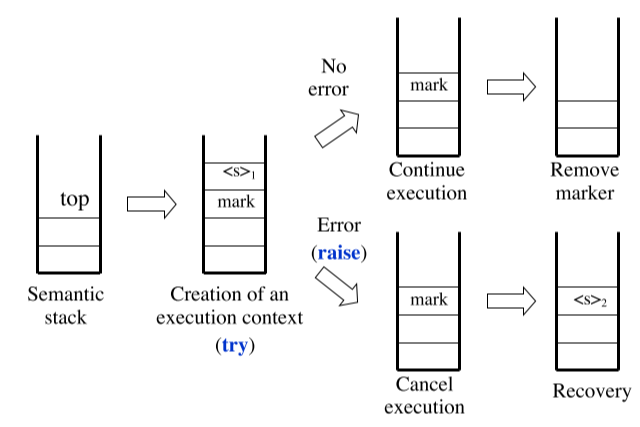
\includegraphics[scale=0.55]{stackException.png}
\end{solution}

\section{The scheduler and its friends}
Define the concept of a scheduler in a concurrent system. Explain precisely what the scheduler does. As part of your explanation, define the six concepts of nondeterminism, time slice, runnable, suspended, fairness, and statvation. Be sure to give a clear definition for each of these six concepts!

\begin{solution}
\begin{itemize}
\item \underline{Scheduler:} partie du système qui décide à tout moment quel thread exécuter (donc exemple non déterminisme)
	\begin{lstlisting}[escapechar=µ]
	declare
	thread X=1 end
	thread X=2 end
	{Browse X} %On ne sait pas si 1 ou 2 sera affichµ\textcolor{gray}{é}µ
	\end{lstlisting}
% oui on doit faire "µ\textcolor{gray}{é}µ" pour afficher un accent mdr
\item \underline{Non déterminisme:} Capacité du système à faire des décisions indépendantes du développeur.
\item \underline{Time slice:} courte période (souvent 10 ms) pendant laquelle s'exécute un thread.
\item \underline{Runnable:} dit d'un thread si l'instruction située au sommet de sa stack n'est pas en attente d'une variable dataflow.
\item \underline{Suspended:} dit d'un thread si il est bloqué sur une variable.
\item \underline{Fairness:} dit d'un scheduler, si chaque runnable thread sera exécuté dans un temps fini (les threads sont classés en fonction de leur priorité et des garanties supplémentes sont données sur le pourcentage du temps accordé aux threads de même priorité)
\item \underline{Starvation:} si le scheduler n'est pas \textit{fair}. Certains threads peuvent "\textit{starve}" donc recevoir 0\% du temps du processeur et ne s'exécutent donc jamais et le programme s'arrête.
\end{itemize}
\end{solution}

\section{Erlang support for fault tolerance}

\subsection{Process linking}
An Erlang process is similar to a port Object. An important primitive operation to support fault tolerance in Erlang is linking, where processes are linked together. For this question, define linking and explain what it does. How does it work when there are more than processes?

\begin{solution}
Link crée un lien entre 2 processus qui est bidirectionnel dans les 2 sens. Lorsqu'un process s'arrête il envoie le signal "normal" à tous les processus auxquels il est lié, sinon il envoie la cause de son arrêt \textit{anormal}. Les processus qui reçoivent un message "anormal" crash aussi et renvoient le message causant le crash.\par 
Un process peut être configuré pour piéger les signaux de sorte en appelant \textit{process\_flag}(trap\_exit, true)\par 
Un superviseur peut recevoir dans sa mailbox le message sans s'arrêter et prendre des mesures pour restaurer le système. \par 
Ainsi, tous les processus liés au crash en suivant la chaine jusqu'à arriver au superviseur. Si aucun process ne démarre, le programme s'arrête. On peut outrepasser un superviseur avec \textbf{exit(kill, Pid)}.
\end{solution}

\subsection{Supervisor trees}
One of the key concepts in Erlang/OTP to support fault tolerance is the supervisor tree. Explain what is a supervisor tree. As part of your answer, give two restart strategies and explain how they work. Justify each strategy with a simple execution scenario.

\begin{solution}
Un arbre de supervision peut redémarrer, modifier ou arrêter un processus qu'il observe (auquel il est lié). Un superviseur, est lui-même supervisé par un autre superviseur, au cas où il échoue. 2 stratégies:
\begin{enumerate}
\item One\_for\_one: quand un des enfants crash, il est simplement redémarré par le superviseur sans que ça n'impacte les autres processus (\textit{ex}: client serveur: pour pas impacter les autres clients si il y a un crash)
\item One\_for\_all: si un des enfants crash, tous les processus liés par le même superviseur sont arrêtés et relancés, même s'ils n'ont aucun problème (\textit{ex}: processus synchronisé: nécessaire quand les processus sont dépendants, pour qu'ils restent synchronisés)
\end{enumerate}
\end{solution}


\end{document}
